%==============================================================================
%  INFORME FINAL - ALGORITMOS Y PROGRAMACION III (ICESI, 2026-1)
%  Clasificacion de calidad y estimacion de tamano de manzanas por vision
%  por computador.
%
%  COMPILAR: subir la carpeta docs/ a Overleaf, clase IEEEtran, pdfLaTeX.
%            Las figuras (PDF vectorial) estan en docs/figures/.
%  Maximo 7 paginas (lineamiento del enunciado).
%==============================================================================
\documentclass[conference]{IEEEtran}
\IEEEoverridecommandlockouts
\usepackage[utf8]{inputenc}
\usepackage[T1]{fontenc}
\usepackage[spanish]{babel}
\usepackage{graphicx}
\usepackage{amsmath,amssymb}
\usepackage{booktabs}
\usepackage{url}
\usepackage{hyperref}
\hypersetup{colorlinks=true,linkcolor=black,citecolor=black,urlcolor=blue}
\graphicspath{{figures/}}

\begin{document}

\title{Clasificación de la calidad y estimación del tamaño de manzanas mediante
visión por computador: comparación de modelos clásicos y una red neuronal
convolucional}

\author{
\IEEEauthorblockN{David Alejandro Troya}
\IEEEauthorblockA{\textit{Algoritmos y Programación III}\\
\textit{Universidad ICESI}, Cali, Colombia\\ troyaalejandro4@gmail.com}
\and
\IEEEauthorblockN{Santiago Morales Cerón}
\IEEEauthorblockA{\textit{Algoritmos y Programación III}\\
\textit{Universidad ICESI}, Cali, Colombia\\ Santiagomorales.c15@gmail.com}
\and
\IEEEauthorblockN{Juan Esteban Gómez Higidio}
\IEEEauthorblockA{\textit{Algoritmos y Programación III}\\
\textit{Universidad ICESI}, Cali, Colombia\\ 09juanesteban@gmail.com}
}
\maketitle

%------------------------------------------------------------------ Resumen
\begin{abstract}
La clasificación manual de la calidad de frutas es lenta, subjetiva y propensa a
errores, lo que genera pérdidas económicas y desperdicio de alimentos. Se
desarrolla un sistema de visión por computador que, a partir de la fotografía de
una manzana, predice su \emph{calidad} (buena, regular, mala) y estima su
\emph{tamaño} (diámetro normalizado y clase pequeño/mediano/grande). Se segmenta
la fruta para calcular un descriptor de 49 características de color, textura y
defectos \emph{solo sobre la fruta} (invariante al fondo), y se comparan, bajo el
mismo protocolo, tres modelos clásicos (regresión logística, SVM-RBF y Random
Forest) y una red neuronal convolucional (CNN). Sobre 3006 imágenes (2890 del
dataset público y 116 propias), los cuatro modelos alcanzaron un desempeño
comparable en prueba (F1-macro 0{,}94--0{,}95); por validación cruzada la SVM-RBF
fue la mejor (0{,}967), muy por encima de la línea base logística (0{,}838). Se sigue
la metodología CRISP-DM y se discuten el sesgo de los datos, la validez de los
resultados y los aspectos éticos.
\end{abstract}
\begin{IEEEkeywords}
visión por computador, clasificación de calidad, segmentación, SVM, Random
Forest, CNN, estimación de tamaño, CRISP-DM.
\end{IEEEkeywords}

%------------------------------------------------------------------ Introduccion
\section{Introducción}
En mercados y agroindustrias, la clasificación de productos frescos según
madurez, tamaño o defectos se hace de forma manual: un proceso lento, subjetivo y
costoso que contribuye a pérdidas y desperdicio de alimentos~\cite{fao}.
Automatizarla con visión por computador permite acelerar el proceso y
estandarizar criterios.

Este proyecto desarrolla un sistema que, dada la foto de una manzana sobre fondo
simple, entrega dos salidas exigidas por el caso de estudio: (i) la \emph{clase
de calidad} en tres categorías (buena, regular, mala) y (ii) una \emph{estimación
de tamaño}. La justificación es directa: reducir pérdidas poscosecha tiene
impacto económico, social y ambiental. El aporte técnico se concentra en un
descriptor de color/textura calculado únicamente sobre la fruta segmentada
(evitando que el modelo aprenda el fondo), la comparación rigurosa de cuatro
modelos y un análisis crítico de la validez de los resultados.

%------------------------------------------------------------------ Fundamentos
\section{Fundamentos teóricos}
\label{sec:fundamentos}
\textbf{Espacio HSV e histogramas.} El color es el principal indicador de calidad
de la fruta. Se trabaja en el espacio HSV, que separa el tono (Matiz) de la
intensidad. El histograma normalizado de un canal, $h_b=\frac{1}{N}\sum_p
\mathbb{1}[c_p\in\text{bin}_b]$, cumple $\sum_b h_b=1$ y es invariante al número
de píxeles (y a la resolución).

\textbf{Estandarización (z-score).} Cada característica se reescala como
$z=(x-\mu)/\sigma$, con $\mu,\sigma$ estimados solo en entrenamiento. Es
necesaria para SVM-RBF, la regresión logística y la red neuronal, sensibles a la
escala.

\textbf{Segmentación y tamaño.} La fruta se separa del fondo con un umbral de
Otsu sobre la distancia al color de fondo (estimado en los bordes). El tamaño se
mide con el diámetro equivalente del área segmentada, $d_{eq}=2\sqrt{A/\pi}$,
normalizado por el lado de la imagen (invariante a la resolución).

\textbf{Modelos.} La \emph{regresión logística} (línea base) modela
$P(y{=}k\,|\,\mathbf{x})$ con softmax. La \emph{SVM} busca el hiperplano de
máximo margen y usa el kernel RBF
$K(\mathbf{x}_i,\mathbf{x}_j)=\exp(-\gamma\lVert\mathbf{x}_i-\mathbf{x}_j\rVert^2)$
para fronteras no lineales~\cite{cortes}. El \emph{Random Forest} promedia
múltiples árboles con muestreo aleatorio, reduciendo la varianza. La \emph{CNN}
aprende filtros sobre los píxeles mediante capas Conv--ReLU--Pooling y minimiza
la entropía cruzada $\mathcal{L}=-\frac1n\sum_i\sum_k y_{ik}\log p_{ik}$ por
retropropagación con Adam~\cite{kingma}.

\textbf{Métricas.} A partir de la matriz de confusión se calculan precisión,
exhaustividad (\emph{recall}) y $F1=2\,PR/(P+R)$ por clase; se reporta el
\textbf{F1-macro} (promedio entre clases), adecuado ante el desbalance, validado
con validación cruzada estratificada de 5 pliegues.

%------------------------------------------------------------------ Formulacion
\section{Formulación matemática del problema}
\label{sec:formulacion}
Sea $I\in[0,1]^{H\times W\times 3}$ la fotografía de una manzana sobre fondo
simple ($H=W=128$). El sistema debe construir dos funciones: un
\emph{clasificador de calidad} $g:I\mapsto y\in\mathcal{Y}=\{\text{buena},
\text{regular},\text{mala}\}$ y un \emph{estimador de tamaño}
$h:I\mapsto(d,\hat s)$, con $d\in[0,1]$ el diámetro normalizado y $\hat
s\in\{\text{pequeño},\text{mediano},\text{grande}\}$.

\textbf{Representación.} Se define $\phi=\phi_2\circ\phi_1$, con
$\phi_1(I)=M\in\{0,1\}^{H\times W}$ la máscara de segmentación (umbral de Otsu,
Sec.~\ref{sec:fundamentos}) y $\phi_2(I,M)=\mathbf{x}\in\mathbb{R}^{49}$ el
descriptor de color/textura/defectos calculado solo sobre $M$. Para los modelos
clásicos $g=f_\theta\circ\phi$; para la CNN, $g=f_\theta$ actúa directamente
sobre $I\odot M$ redimensionada a $64\times64$, de modo que $\phi$ es la
identidad enmascarada y la representación se \emph{aprende} dentro de
$f_\theta$ en lugar de diseñarse a mano.

\textbf{Aprendizaje como minimización del riesgo empírico regularizado.} Dado
$D=\{(\mathbf{x}_i,y_i)\}_{i=1}^{n}$ ($n=2104$), se busca
\[
\theta^\ast=\arg\min_{\theta\in\Theta}\ \frac{1}{n}\sum_{i=1}^{n}
w_{y_i}\,\mathcal{L}\big(f_\theta(\mathbf{x}_i),y_i\big)+\lambda\,R(\theta),
\]
donde $f_\theta:\mathbb{R}^{49}\to\Delta^{2}$ (o
$f_\theta:[0,1]^{64\times64\times3}\to\Delta^{2}$ en la CNN) entrega una
distribución sobre las 3 clases, $\mathcal{L}$ es la entropía cruzada de la
Sec.~\ref{sec:fundamentos}, $w_{y_i}=n/(3\,n_{y_i})$ son los pesos balanceados
de clase (compensan el desbalance 1197/638/1171), $R$ es el regularizador
propio de cada familia ($\ell_2$ en regresión logística; margen y par
$(C,\gamma)$ del kernel en SVM-RBF; profundidad y número de árboles en Random
Forest; arquitectura y \emph{weight decay} en la CNN) y $\Theta$ es el espacio
de hipótesis correspondiente.

\textbf{Selección de modelo e hiperparámetros (optimización de segundo
nivel).} Se resuelve por búsqueda en rejilla con validación cruzada
estratificada de 5 pliegues, maximizando el F1-macro de la
Sec.~\ref{sec:fundamentos}:
\[
(m^\ast,\lambda^\ast)=\arg\max_{(m,\lambda)\in\mathcal{M}\times\Lambda}\
\frac{1}{5}\sum_{k=1}^{5} F1_{\text{macro}}\big(f^{(m,\lambda)};
D^{(k)}_{\text{val}}\big),
\]
con $\mathcal{M}=\{\text{LogReg},\text{SVM-RBF},\text{RF},\text{CNN}\}$ y
$\Lambda$ la rejilla propia de cada familia (resultado: $m^\ast=$ SVM-RBF,
Tabla~\ref{tab:res}). Nótese que este es un problema de optimización anidado:
para cada $(m,\lambda)$ candidato se resuelve internamente el problema de
minimización de $\theta$ descrito arriba.

\textbf{Estimación de tamaño (medición, no aprendizaje).} A partir de
$M=\phi_1(I)$ se mide el diámetro equivalente normalizado
$d=2\sqrt{A/\pi}\,/\sqrt{HW}$, $A=\sum_{p}M_p$ (Sec.~\ref{sec:fundamentos}), y
se discretiza con umbrales $\tau_1,\tau_2$ calibrados sobre la distribución
empírica del conjunto: $\hat s=$ pequeño si $d<\tau_1$, mediano si
$\tau_1\le d<\tau_2$, grande si $d\ge\tau_2$, con $\tau_1=0{,}45$ y
$\tau_2=0{,}62$.

\textbf{¿Por qué es un problema complejo de ingeniería?} (a) $g$ debe
aproximar una función no lineal de alta dimensión —$128\times128\times3=49152$
variables de entrada— hacia 3 clases, sin una regla cerrada conocida; (b) hay
que resolver \emph{a la vez} un problema de representación ($\phi$: qué
calcular) y uno de aprendizaje ($f_\theta$: qué ajustar) que interactúan entre
sí —la Sec.~\ref{sec:analisis} muestra que omitir la máscara en $\phi$ produce
una métrica artificialmente alta e inválida (fuga de información del fondo)—;
(c) las clases están desbalanceadas y la clase \emph{regular} se construyó de
forma sintética, lo que obliga a introducir $w_{y_i}$ y validación
estratificada; (d) coexisten cuatro espacios de hipótesis con geometrías y
costos de búsqueda distintos, y compararlos limpiamente exige fijar partición,
semilla, estandarización y métrica (Sec.~\ref{sec:metodologia}); (e) la
estimación de tamaño añade una tarea de \emph{medición geométrica}
(segmentación y calibración de $\tau_1,\tau_2$) acoplada a la de clasificación.
Esta formulación conecta directamente con el objetivo del proyecto: producir,
a partir de una sola fotografía, las dos salidas exigidas por el caso de
estudio bajo un protocolo de comparación reproducible y honesto.

%------------------------------------------------------------------ Metodologia
\section{Metodología}
\label{sec:metodologia}
Se aplicó CRISP-DM (Fig.~\ref{fig:crisp}) con evidencia en cada fase. La
formulación de la Sec.~\ref{sec:formulacion} guía cada decisión: qué calcular
($\phi$), qué familias de modelos comparar ($\mathcal{M}$) y con qué criterio
elegir ($F1_{\text{macro}}$ por validación cruzada).

\begin{figure*}[t]
\centering
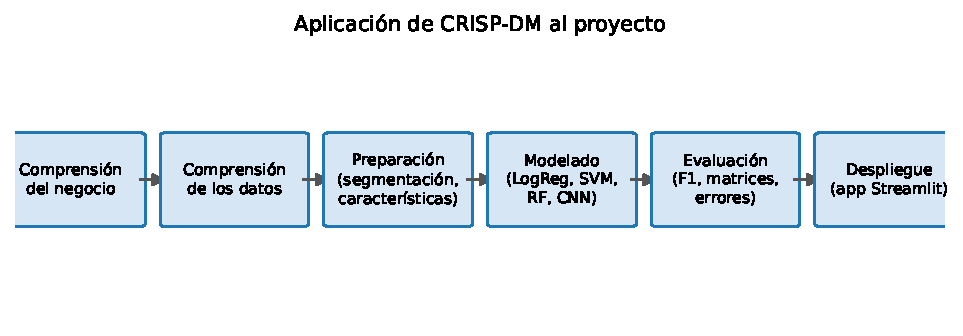
\includegraphics[width=0.92\textwidth]{fig_crispdm.pdf}
\caption{Aplicación concreta de CRISP-DM al proyecto.}
\label{fig:crisp}
\end{figure*}

\textbf{Datos.} Se usó el conjunto público \emph{Fruit Quality Classification}
de Kaggle~\cite{kaggle}, subconjunto de manzanas: \emph{buena} (1149,
\textit{Apple\_Good}) y \emph{mala} (1141, \textit{Apple\_Bad}). La clase
\emph{regular} se construyó, según indica el caso de estudio, segmentando
individualmente cada fruta de la carpeta \textit{Mixed Quality} (177 ejemplares
recortados) y aumentándola con transformaciones (volteos, rotaciones, brillo)
hasta 600 muestras para reducir el desbalance. Además, se recolectaron y
añadieron \textbf{116 fotografías propias} tomadas para este proyecto (48 sanas,
38 intermedias y 30 dañadas), como exige el caso de estudio, integradas a las
tres clases. En total, \textbf{3006 imágenes} (buena 1197, regular 638, mala
1171). Las Figs.~\ref{fig:dist} muestran la distribución de calidad y tamaño.

\begin{figure}[t]
\centering
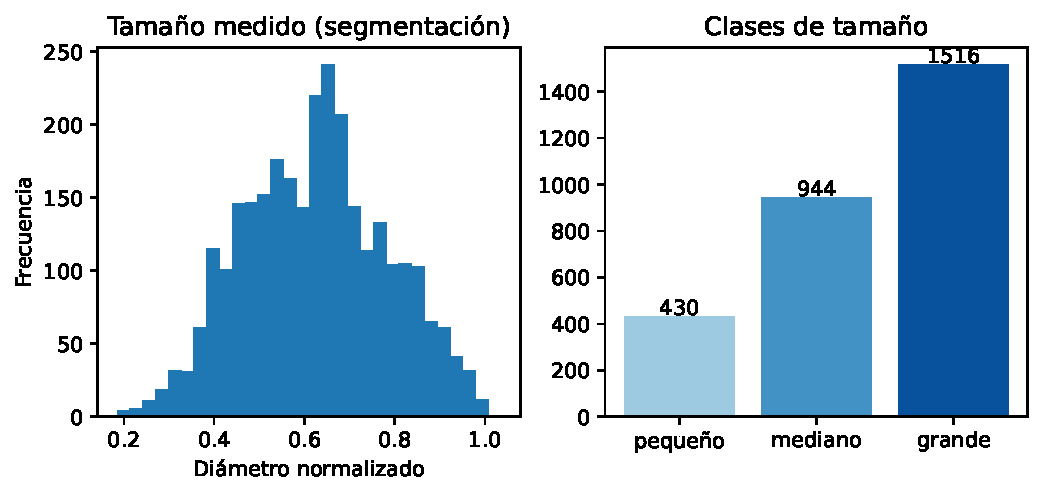
\includegraphics[width=0.95\columnwidth]{fig_size_distribution.pdf}\\[2pt]
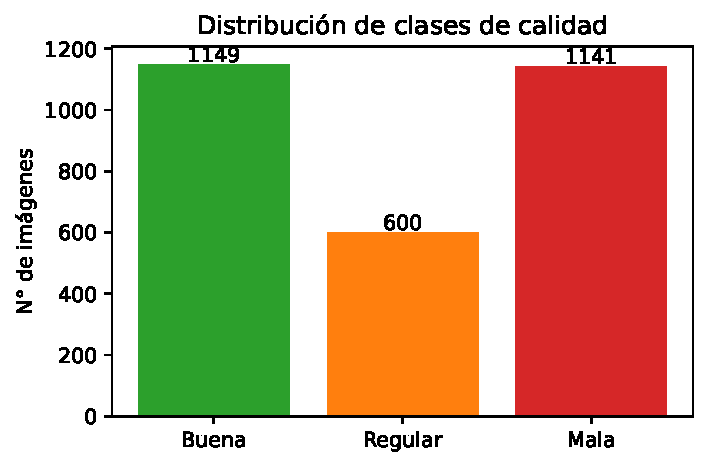
\includegraphics[width=0.62\columnwidth]{fig_class_distribution.pdf}
\caption{Distribución del tamaño medido (arriba) y de las clases de calidad
(abajo).}
\label{fig:dist}
\end{figure}

\textbf{Preparación y características.} Cada imagen se redimensiona a $128\times
128$ (elimina el sesgo de resolución) y se segmenta la fruta
(Fig.~\ref{fig:seg}). Sobre los píxeles de la fruta se calcula un vector de
\textbf{49 características}: histogramas de H/S/V (16/8/8), media y desviación de
R,G,B,H,S,V (12), estadísticos de gradiente (2, textura), proporción de píxeles
oscuros y marrones (2, defectos) y entropía de matiz (1). \emph{Calcular las
características solo sobre la fruta es una decisión clave}: evita que los modelos
aprendan el fondo (césped, mano, mesa) en lugar de la calidad.

\begin{figure}[t]
\centering
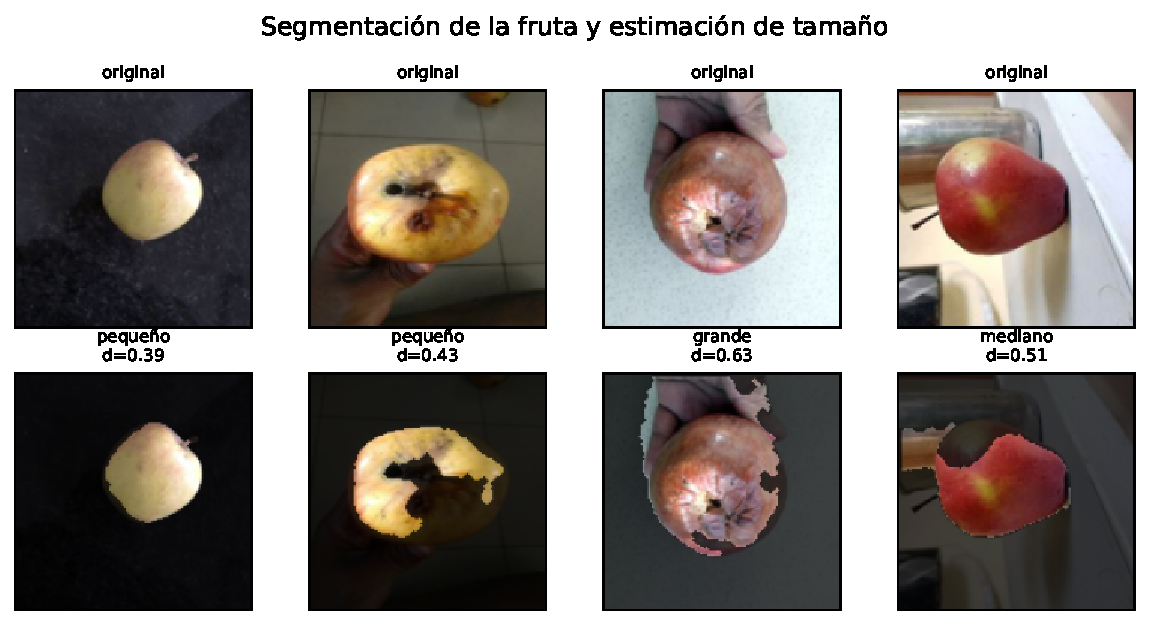
\includegraphics[width=0.98\columnwidth]{fig_segmentation.pdf}
\caption{Segmentación de la fruta y estimación de tamaño (diámetro normalizado).}
\label{fig:seg}
\end{figure}

\textbf{Estrategia de solución y alternativas consideradas.} La formulación
(Sec.~\ref{sec:formulacion}) deja dos preguntas abiertas: (1) ¿basta un
descriptor diseñado a mano de 49 variables, o se necesita aprender la
representación directamente de los píxeles?, y (2) sobre ese descriptor, ¿qué
\emph{forma} de frontera de decisión —lineal, de margen máximo no lineal, o de
comité de árboles— ajusta mejor $g$? En lugar de asumir una respuesta, se
comparan bajo el mismo protocolo cuatro hipótesis representativas:
\emph{regresión logística} como \textbf{línea base} lineal e interpretable —si
un modelo no lineal no la supera con claridad, no se justifica su mayor costo—;
\emph{SVM-RBF}, que mediante el kernel $K$ (Sec.~\ref{sec:fundamentos})
construye fronteras no lineales en espacios de pocas decenas de dimensiones sin
requerir datasets masivos, el escenario típico de un descriptor diseñado a
mano~\cite{cortes}; \emph{Random Forest}, robusto a variables en escalas y
correlaciones distintas (como ocurre entre histogramas de color contiguos),
que reduce varianza promediando árboles y, a diferencia de SVM y CNN, entrega
\emph{importancia de características} (Fig.~\ref{fig:imp}) útil para validar
si el modelo aprende señales agronómicamente sensatas; y una \emph{CNN}
pequeña (3 bloques convolucionales + 2 capas densas, entrada $64\times64$
enmascarada, Adam, entropía cruzada con pesos~\cite{kingma}), incluida como
contraste directo de la hipótesis alternativa (1): aprender $\phi$ en lugar de
diseñarlo. Se descartaron explícitamente \emph{KNN} (sensible a la maldición de
la dimensionalidad y a la correlación entre histogramas adyacentes),
\emph{Gradient Boosting} (espacio de hiperparámetros más amplio y mayor riesgo
de sobreajuste dado el tamaño moderado y el desbalance del dataset, sin ganancia
esperada sobre Random Forest) y arquitecturas profundas preentrenadas
(\emph{transfer learning} tipo ResNet/EfficientNet, descartadas por la
simplicidad del fondo y el tamaño del conjunto; se documentan como trabajo
futuro).

Para que la comparación sea válida —y la elección del ganador, defendible— se
fijaron partición estratificada 70/30 (2104 entrenamiento, 902 prueba, semilla
42), estandarización ajustada \emph{solo} en entrenamiento,
\texttt{class\_weight} balanceado ($w_{y_i}$ de la Sec.~\ref{sec:formulacion})
y un único criterio de selección automática: el F1-macro en validación cruzada
estratificada de 5 pliegues, que \emph{no} usa el conjunto de prueba —evita que
la elección del modelo esté contaminada por los datos sobre los que luego se
informa el desempeño final—.

\textbf{Despliegue.} Aplicación en Streamlit que permite cargar una imagen o
capturarla con la cámara y muestra calidad, tamaño y segmentación.

%------------------------------------------------------------------ Resultados
\section{Resultados}
La Tabla~\ref{tab:res}, la Tabla~\ref{tab:pc} y la Fig.~\ref{fig:cmp} resumen el
desempeño. El modelo se selecciona por validación cruzada (sin usar el conjunto
de prueba): la \textbf{SVM-RBF fue la mejor (F1-macro CV 0{,}967)}, seguida de
Random Forest (0{,}950) y la regresión logística (0{,}856). En el conjunto de
prueba los tres mejores modelos quedaron \emph{prácticamente empatados} (SVM
0{,}949, CNN 0{,}953, Random Forest 0{,}944), muy por encima de la línea base
(0{,}838); la cercanía entre CV y prueba indica ausencia de sobreajuste severo. Las matrices de
confusión (Fig.~\ref{fig:cm}) muestran que los errores se concentran entre
\emph{buena} y \emph{mala}. La importancia de características
(Fig.~\ref{fig:imp}) confirma que los descriptores de color (saturación y matiz)
son los más decisivos, coherente con la intuición agronómica. La proyección PCA
(Fig.~\ref{fig:pca}) muestra clases separables con zonas de solape, y la
Fig.~\ref{fig:ex} ilustra predicciones de calidad y tamaño.

\begin{table}[t]
\caption{Resultados globales ($n_{prueba}=902$). El mejor modelo se elige por
F1-macro en validación cruzada (CV).}
\label{tab:res}
\centering
\begin{tabular}{lccc}
\toprule
Modelo & Exactitud & F1-macro & F1-macro CV \\
\midrule
Regresión logística & 0.837 & 0.838 & 0.856 \\
\textbf{SVM (RBF)}  & 0.948 & 0.949 & \textbf{0.967} \\
Random Forest       & 0.943 & 0.944 & 0.950 \\
CNN (3 conv.)       & 0.951 & 0.953 & --- \\
\bottomrule
\end{tabular}
\end{table}

\begin{table}[t]
\caption{F1 por clase (prueba).}
\label{tab:pc}
\centering
\begin{tabular}{lccc}
\toprule
Modelo & Buena & Regular & Mala \\
\midrule
Reg. logística & 0.82 & 0.84 & 0.85 \\
SVM (RBF)      & 0.94 & 0.96 & 0.95 \\
Random Forest  & 0.94 & 0.95 & 0.95 \\
CNN            & 0.94 & 0.96 & 0.95 \\
\bottomrule
\end{tabular}
\end{table}

\begin{figure}[t]
\centering
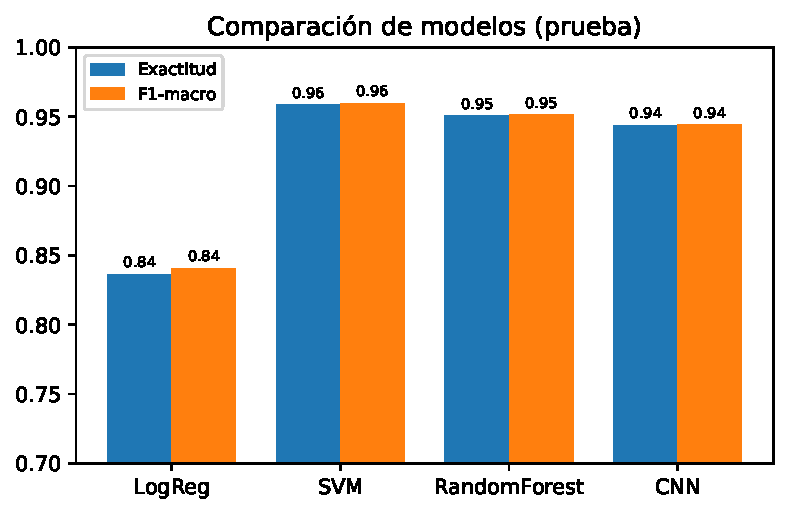
\includegraphics[width=0.95\columnwidth]{fig_model_comparison.pdf}
\caption{Comparación de los cuatro modelos.}
\label{fig:cmp}
\end{figure}

\begin{figure}[t]
\centering
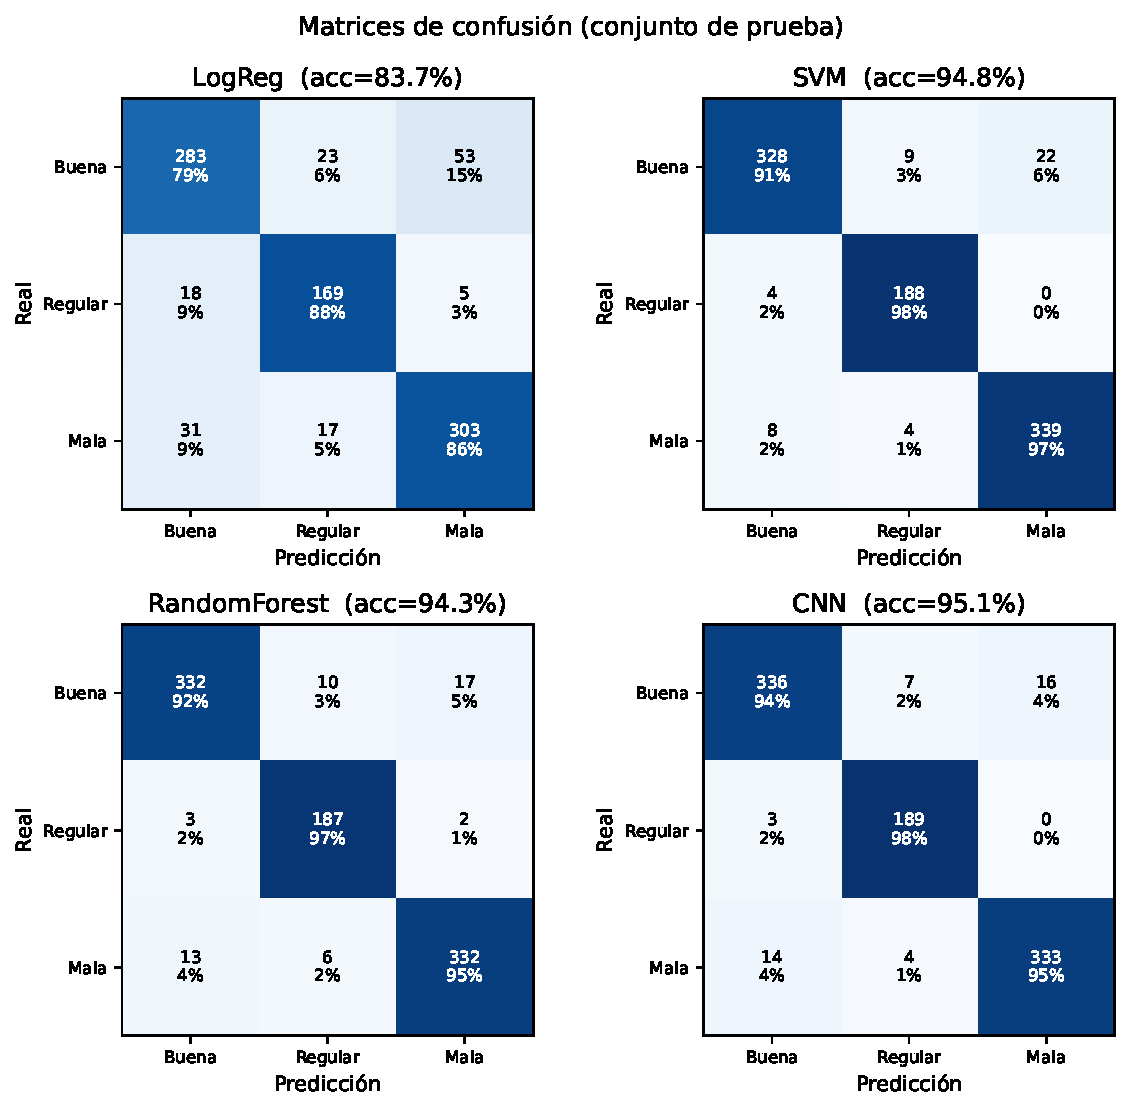
\includegraphics[width=0.99\columnwidth]{fig_confusions.pdf}
\caption{Matrices de confusión normalizadas (prueba).}
\label{fig:cm}
\end{figure}

\begin{figure}[t]
\centering
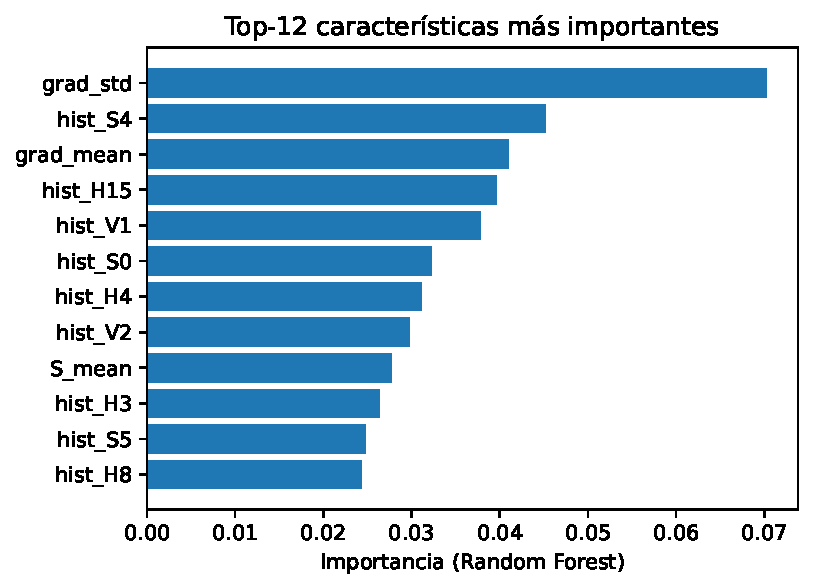
\includegraphics[width=0.92\columnwidth]{fig_feature_importance.pdf}
\caption{Importancia de características (Random Forest).}
\label{fig:imp}
\end{figure}

%------------------------------------------------------------------ Analisis
\section{Análisis de resultados}
\label{sec:analisis}
\textbf{¿Generalizan? ¿Hay sobreajuste?} La cercanía entre CV y prueba indica que
los modelos generalizan dentro de este dataset, sin sobreajuste marcado.
\emph{Los tres mejores modelos son estadísticamente comparables} (diferencias
$<$1 punto en prueba): la CNN, que aprende de los píxeles, y los modelos clásicos
(SVM y Random Forest), que usan características diseñadas a mano, alcanzan
resultados equivalentes. Esto sugiere que, a esta escala de datos, las
características de color son muy informativas y una CNN pequeña no aporta una
ventaja clara. Se reporta la SVM como mejor modelo por su F1-macro en validación
cruzada, el criterio de selección que no usa el conjunto de prueba.

\textbf{¿Qué funciona y qué falla?} El sistema separa muy bien la fruta podrida
(color marrón/oscuro) de la sana; los errores residuales ocurren entre buena y
mala con iluminación o manchas ambiguas. Segmentar y usar características solo de
la fruta fue decisivo: en una versión previa con el fondo incluido, la clase
\emph{regular} alcanzaba un 100\% irreal porque el modelo reconocía el fondo de
los recortes; al enmascarar el fondo, la métrica bajó a valores realistas
(0{,}96) y honestos.

\textbf{Limitaciones.} (i) La clase \emph{regular} se construyó con recortes
segmentados de la carpeta \textit{Mixed} y aumento de datos, por lo que es menos
diversa. (ii) Las imágenes provienen de un único dataset; el desempeño podría
caer con cámaras, iluminación o variedades distintas (cambio de dominio). (iii)
La estimación de tamaño depende de la calidad de la segmentación y de un fondo
simple; sin referencia de escala, entrega un diámetro \emph{relativo}, no
absoluto. (iv) La segmentación (Sec.~\ref{sec:fundamentos}) asume una sola
fruta como objeto dominante: selecciona la componente conexa más grande que
contrasta con el fondo, sin verificar que en efecto sea una manzana; con varias
frutas, fondos complejos o presencia de otros objetos puede aislar (y por
tanto clasificar) algo distinto de la manzana. (v) En la literatura, FruitNet
reporta exactitudes del orden de
85--95\,\% con CNN; nuestros resultados son comparables, recordando que el dato
es relativamente ``limpio''.

%------------------------------------------------------------------ Etica e impactos
\section{Aspectos éticos e impactos}
\label{sec:etica}
\textbf{Dilemas éticos identificados y decisiones tomadas, en relación directa
con los principios del \emph{ACM Code of Ethics and Professional
Conduct}~\cite{acm} (versión adoptada también por IEEE-CS).}

\emph{Sesgo y equidad} (Principio 1.4, ``ser justo y no discriminar''): un
modelo entrenado sobre un dataset de origen único (variedad, iluminación y
cámara del conjunto de Kaggle) puede generalizar mal —y resultar injusto— con
frutas de otros productores, regiones o condiciones de cultivo, perjudicando
económicamente a quien lo use. \textbf{Decisión adoptada:} documentar el sesgo
explícitamente (ver Limitaciones) y ampliar el conjunto con 116 fotografías
propias, capturadas en condiciones distintas a las del dataset original, como
medida concreta y reproducible de mitigación.

\emph{Privacidad y consentimiento} (Principios 1.6 ``respetar la privacidad'' y
1.7 ``honrar la confidencialidad''): varias fotografías —tanto del dataset
público como las propias— muestran manos o superficies que podrían identificar
a una persona o un lugar. \textbf{Decisión adoptada:} (a) las fotografías
propias fueron tomadas y aportadas por los mismos autores, quienes consintieron
expresamente su uso académico y su publicación en el repositorio del curso; (b)
no se almacenan ni publican metadatos personales (geolocalización, EXIF,
nombres); (c) la segmentación recorta el fondo \emph{antes} de calcular
características, lo que de paso reduce la información personal retenida en el
pipeline de cómputo.

\emph{Honestidad académica e integridad} (Principios 1.3 ``ser honesto y
confiable'' y 2.5 ``dar evaluaciones completas y objetivas''): se decidió
reportar, en vez de omitir, el episodio en que la clase \emph{regular} alcanzó
un F1 irreal de 100\,\% por una fuga de información del fondo
(Sec.~\ref{sec:analisis}), y elegir el modelo final por validación cruzada
—nunca por el conjunto de prueba— para no inflar artificialmente la cifra que
se reporta. Se referencian explícitamente el dataset de
terceros~\cite{kaggle} y las bibliotecas usadas~\cite{scikit}.

\emph{Uso responsable y prevención de daño} (Principio 1.2 ``evitar daño''):
una predicción errónea de calidad tiene costo económico (descartar fruta sana)
o sanitario (aceptar fruta en mal estado). \textbf{Decisión adoptada:}
presentar el sistema como \emph{herramienta de apoyo a la decisión humana}, no
como reemplazo de un clasificador experto; publicar el F1 por clase
(Tabla~\ref{tab:pc}) para que cualquier usuario sepa en qué clase el sistema es
menos confiable; y documentar explícitamente el supuesto de operación —una
sola fruta sobre fondo simple— y sus consecuencias (párrafo de Limitaciones,
Sec.~\ref{sec:analisis}),
de modo que quien despliegue o evalúe el sistema entienda \emph{cuándo} confiar
menos en la predicción (p.\ ej., con varias frutas u objetos ajenos en la
imagen, la segmentación puede describir algo distinto de la manzana).

La Tabla~\ref{tab:etica} resume estos cuatro dilemas, el principio concreto del
código de ética que cada uno involucra y la medida adoptada en el proyecto.

\begin{table}[t]
\caption{Dilemas éticos identificados, principio del código ACM/IEEE
involucrado y medida concreta adoptada en el proyecto.}
\label{tab:etica}
\centering
\begin{tabular}{p{1.7cm}p{2.6cm}p{3.1cm}}
\toprule
Dilema & Principio (ACM/IEEE~\cite{acm}) & Medida adoptada \\
\midrule
Sesgo de origen único & 1.4 Ser justo y no discriminar & Documentar el sesgo;
ampliar el dataset con 116 fotos propias en condiciones distintas \\
Privacidad / consentimiento & 1.6 Privacidad; 1.7 Confidencialidad &
Fotos propias con consentimiento expreso de los autores; sin metadatos
personales; recorte del fondo antes de procesar \\
Honestidad académica & 1.3 Honestidad; 2.5 Evaluación objetiva y completa &
Reportar la fuga de información detectada; seleccionar por CV (no por prueba);
citar fuentes de datos y software \\
Riesgo de daño / uso responsable & 1.2 Evitar daño & Presentar el sistema como
apoyo a la decisión humana; publicar F1 por clase; documentar el supuesto de
operación (una fruta, fondo simple) y sus límites \\
\bottomrule
\end{tabular}
\end{table}

\textbf{Análisis de impactos y estrategias de mitigación.} La Tabla~\ref{tab:impactos}
resume, para cada dimensión exigida por la guía, el argumento técnico-ético y la
estrategia concreta propuesta para potenciar los beneficios y mitigar los
riesgos.

\begin{table}[t]
\caption{Matriz de impactos: análisis por dimensión y estrategia de
mitigación/potenciación propuesta.}
\label{tab:impactos}
\centering
\begin{tabular}{p{1.3cm}p{3.0cm}p{3.1cm}}
\toprule
Dimensión & Análisis (beneficio / riesgo) & Estrategia propuesta \\
\midrule
Económico & Reduce el descarte de fruta vendible y agiliza la clasificación;
pero un falso ``mala'' desecha producto sano y un falso ``buena'' puede dañar
la reputación del vendedor (Tabla~\ref{tab:pc} cuantifica ese riesgo por clase)
& Calibrar el umbral de decisión según el costo asimétrico del caso de uso y
mantener supervisión humana en las predicciones de menor confianza \\
Ambiental & Menos desperdicio implica ahorrar el agua, el suelo y la energía ya
invertidos en la fruta descartada (huella evitada); los modelos clásicos
corren en CPU, con bajo consumo frente a redes profundas grandes &
Preferir en producción el modelo clásico (SVM o Random Forest) sobre la CNN
cuando el desempeño sea equivalente —como ocurre aquí (Tabla~\ref{tab:res})—,
pues reduce el cómputo y la huella de carbono del despliegue \\
Social & Estandariza un criterio hoy subjetivo y reduce la exposición de
operarios a tareas repetitivas; pero puede desplazar empleo de clasificación
manual & Comunicar el sistema como herramienta de \emph{apoyo} (no reemplazo,
como se argumentó arriba) y acompañar su adopción con programas de
recapacitación hacia tareas de supervisión y control de calidad \\
Global & Contribuye a los Objetivos de Desarrollo Sostenible 2 (Hambre cero) y
12 (Producción y consumo responsables)~\cite{onu}, al atacar directamente las
pérdidas poscosecha que documenta la FAO~\cite{fao} & Publicar el código y el
modelo (Sec. Enlaces) para que comunidades agrícolas de otras regiones lo
adapten a sus propias variedades, mitigando a la vez el sesgo de origen único \\
\bottomrule
\end{tabular}
\end{table}

%------------------------------------------------------------------ Conclusiones
\section{Conclusiones y trabajo futuro}
Se construyó un sistema reproducible que clasifica la calidad de la manzana en
tres clases y estima su tamaño, comparando cuatro modelos bajo el mismo
protocolo. La \textbf{SVM-RBF sobre características de la fruta segmentada} fue el
mejor modelo por validación cruzada (F1-macro 0{,}967), con la CNN y Random Forest
a un nivel equivalente en el conjunto de prueba ($\approx$0{,}95). El mayor
aprendizaje fue metodológico: \emph{segmentar y medir solo la fruta evita un sesgo
de fondo que inflaba artificialmente las métricas}. Como trabajo futuro: ampliar y diversificar el dataset (más fotos
propias y otras variedades, condiciones de captura distintas), usar transferencia
de aprendizaje, segmentación
con redes (U-Net) y una referencia de escala para obtener tamaño absoluto.

\begin{figure}[t]
\centering
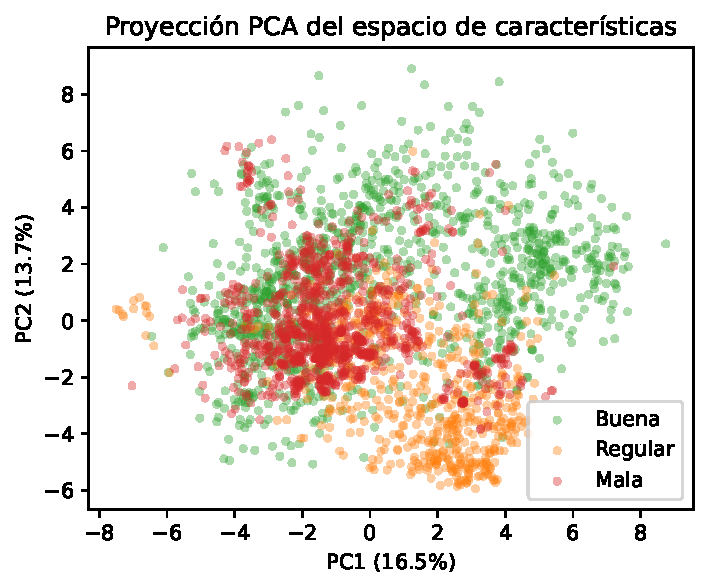
\includegraphics[width=0.82\columnwidth]{fig_pca.pdf}
\caption{Proyección PCA del espacio de características.}
\label{fig:pca}
\end{figure}

\begin{figure}[t]
\centering
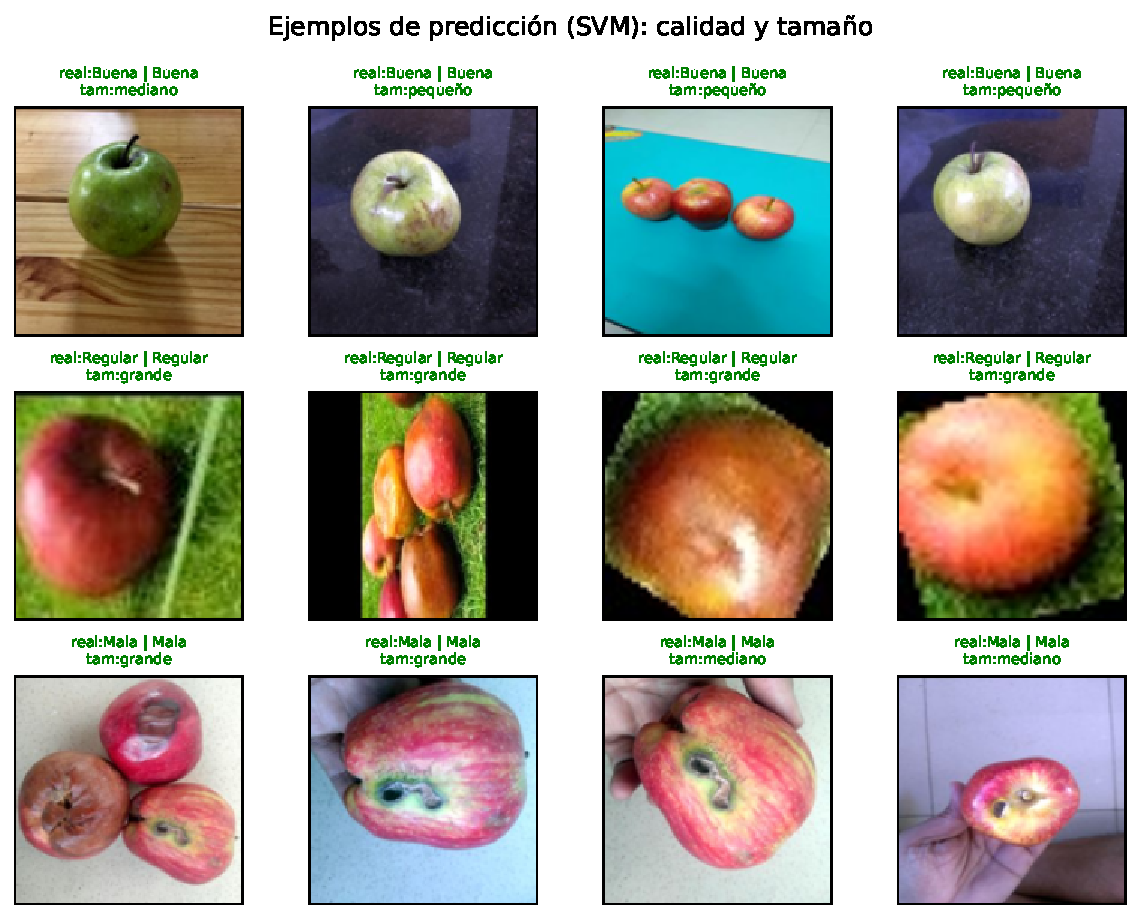
\includegraphics[width=0.99\columnwidth]{fig_examples.pdf}
\caption{Ejemplos de predicción de calidad y tamaño (SVM).}
\label{fig:ex}
\end{figure}

\section*{Enlaces}
\noindent\textbf{Video (máx. 10 min):} \url{https://youtu.be/27Uq-99Mdik}\\
\textbf{Repositorio (código documentado):}
\url{https://github.com/JEGH18/ProyectoFinalAPO3}

\begin{thebibliography}{9}
\bibitem{fao} FAO, ``Pérdidas y desperdicio de alimentos,'' 2019.
\bibitem{onu} Naciones Unidas, ``Objetivos de Desarrollo Sostenible,'' 2015.
[En línea]. \url{https://www.un.org/sustainabledevelopment/es/}
\bibitem{kaggle} R. Park, ``Fruit Quality Classification,'' Kaggle, 2023.
[En línea]. \url{https://www.kaggle.com/datasets/ryandpark/fruit-quality-classification}
\bibitem{cortes} C. Cortes y V. Vapnik, ``Support-vector networks,'' \textit{Machine
Learning}, vol. 20, no. 3, pp. 273--297, 1995.
\bibitem{kingma} D. P. Kingma y J. Ba, ``Adam: A method for stochastic
optimization,'' \textit{ICLR}, 2015.
\bibitem{scikit} F. Pedregosa \textit{et al.}, ``Scikit-learn: Machine learning in
Python,'' \textit{JMLR}, vol. 12, pp. 2825--2830, 2011.
\bibitem{acm} ACM, ``ACM Code of Ethics and Professional Conduct,'' 2018.
\end{thebibliography}

\end{document}
